\title{Solving a Cosserat Rod Initial Value Problem}
\author{John Till}
\date{}

\documentclass[12pt]{article}

\usepackage[a4paper, margin=0.75in]{geometry}
\usepackage[colorlinks=true,urlcolor=blue]{hyperref}
\usepackage{amsmath,amssymb}
\usepackage{graphicx}

\usepackage{xcolor}
\definecolor{OffWhite}{rgb}{0.93,0.93,0.93}
\definecolor{QtCommentColor}{rgb}{0,0.5,0}
\definecolor{QtKeywordColor}{rgb}{0.5,0.5,0}
\definecolor{QtPurpleColor}{rgb}{0.5,0,0.5}
\definecolor{QtGlobal}{rgb}{0.808,0.361,0}
\definecolor{QtFunctionColor}{rgb}{0,0.404,0.486}

\usepackage[T1]{fontenc} %for upquotes in listings
\usepackage{textcomp} %for upquotes in listings
\usepackage{listings}
\lstset{
		language=C++,
		escapeinside={!-}{-!},
		upquote=true,
		%
		otherkeywords={Vector3d, DiagonalMatrix, VectorXd, Matrix3d, Map, MatrixXd,
									UnitX, pow, inverse, transpose, segment, data, UnitZ, cross, hat,
									Zero, Identity, UnitY, cosseratRodOde, ode4, col, row, main, plot},
    morekeywords=[2]{Vector3d, DiagonalMatrix, VectorXd, Matrix3d, Map, MatrixXd},
		morekeywords=[3]{UnitX, UnitZ, pow, inverse, transpose, segment, data, cross, hat,
		                 Zero, Identity, UnitY, cosseratRodOde, ode4, col, row, main, plot},
    %
		frame = single,
		rulecolor=\color{black},
    tabsize=4, % tab space width
    showstringspaces=false, % don't mark spaces in strings
		%
		basicstyle=\footnotesize,%\color{QtIdentifier},
		backgroundcolor=\color{OffWhite},
    commentstyle=\color{QtCommentColor}, % comment color
    keywordstyle=\color{QtKeywordColor}, % keyword color
		keywordstyle=[2]{\color{QtPurpleColor}},
		keywordstyle=[3]{\color{QtFunctionColor}},
    stringstyle=\color{QtCommentColor} % string color
}

\begin{document}

\makeatletter
\renewcommand{\@maketitle}{
\newpage
\null
\vskip 2em
\begin{center}
{\LARGE \@title \par}
\end{center}
\par
} \makeatother

\maketitle

The Cosserat rod equations are stated and then simulated. For more detail on the context of what variables represent and how the equations are derived, see Chapter 2 of Caleb's dissertation \href{https://etd.library.vanderbilt.edu//available/etd-10042011-115347/}{``The Mechanics of Continuum Robots: Model-based Sensing and Control''}. The shape and internal loading of the elastic rod vary along the rod's arc length $s$ as described by the following set of nonlinear ODEs, which are derivatives with respect to the arc length $s$:
\begin{align*}
\dot{\boldsymbol{p}}(s) &= \boldsymbol{R} \boldsymbol{v} \\
\dot{\boldsymbol{R}}(s) &= \boldsymbol{R} \widehat{\boldsymbol{u}} \\
\dot{\boldsymbol{n}}(s) &= -\rho A \boldsymbol{g} \\
\dot{\boldsymbol{m}}(s) &= - \dot{\boldsymbol{p}} \times \boldsymbol{n}
\end{align*}
with the algebraic equations
\begin{align*}
\boldsymbol{v} &= \boldsymbol{e}_3 + \boldsymbol{K}_{se} \boldsymbol{R}^T \boldsymbol{n} \\
\boldsymbol{u} &= \boldsymbol{K}_{bt} \boldsymbol{R}^T \boldsymbol{m},
\end{align*}
where the stiffness matrices above are defined by
\begin{align*}
\boldsymbol{K}_{se} = \begin{bmatrix} GA & 0 & 0 \\ 0 & GA & 0 \\ 0 & 0 & EA \end{bmatrix}, \;\;\;\;
\boldsymbol{K}_{bt} = \begin{bmatrix} EI & 0 & 0 \\ 0 & EI & 0 \\ 0 & 0 & GJ \end{bmatrix}
\end{align*}
and the $\widehat{\cdot}$ symbol is an operator defined by
\begin{align*}
\widehat{\boldsymbol{u}} := \begin{bmatrix} 0 & -u_z & u_y \\ u_z & 0 & -u_x \\ -u_y & u_x & 0 \end{bmatrix}.
\end{align*}
$\rho$, $A$, $I$, $J$, $E$, and $G$ are constant scalar parameters. $\boldsymbol{g}$ is the 3x1 gravitational acceleration vector, also a constant parameter.

The first step in implementing a simulation is to set the constant parameters. That's why the C++ file starts with the lines
\begin{lstlisting}
//Independent Parameters
const double E = 200e9;
const double G = 80e9;
const double rad = 0.001;
const double rho = 8000;
const Vector3d g = 9.81*Vector3d::UnitX();
const double L = 0.5;

//Dependent parameter calculations
const double A = pi*pow(rad,2);
const double I = pi*pow(rad,4)/4;
const double J = 2*I;
const DiagonalMatrix<double, 3> Kse = DiagonalMatrix<double, 3>(G*A,G*A,E*A);
const DiagonalMatrix<double, 3> Kbt = DiagonalMatrix<double, 3>(E*I,E*I,G*J);
\end{lstlisting}
There's nothing too surprising here. The syntax for Eigen matrices might take a little getting used to, but in this snippet we're just setting $\boldsymbol{g} = 9.81*\begin{bmatrix} 1 & 0 & 0 \end{bmatrix}^T$ and using diagonal matrix data structures for the stiffness matrices. The tail part of the ``Vector3d'' name specifies a 3x1 vector of doubles. The constant ``pi'' is defined in ``commonmath.h'' in the library folder.

The next step is to write a function for the ordinary differential equation (ODE). The state variables include 3x1 vectors $\boldsymbol{p}$, $\boldsymbol{n}$, and $\boldsymbol{m}$, as well as the 3x3 rotation matrix $\boldsymbol{R}$. Typically when numerically solving an initial value problem (IVP), all the state variables are combined into a single state vector. For example, we will define the state vector as
\begin{align*}
\boldsymbol{y} := \begin{bmatrix} \boldsymbol{p} \\ \boldsymbol{R}_\text{col1} \\ \boldsymbol{R}_\text{col2} \\ \boldsymbol{R}_\text{col3} \\ \boldsymbol{n} \\ \boldsymbol{m} \end{bmatrix},
\end{align*}
which is an 18x1 vector. Then we write a function to calculate $\dot{\boldsymbol{y}} = f(\boldsymbol{y})$. Our C++ code is:
\begin{lstlisting}
//Ordinary differential equation describing elastic rod
VectorXd cosseratRodOde(VectorXd y){
    //Unpack state vector
    Matrix3d R = Map<Matrix3d>(y.segment<9>(3).data());
    Vector3d n = y.segment<3>(12);
    Vector3d m = y.segment<3>(15);

    //Hard-coded material constitutive equation w/ no precurvature
    Vector3d v = Kse.inverse()*R.transpose()*n + Vector3d::UnitZ();
    Vector3d u = Kbt.inverse()*R.transpose()*m;

    //ODEs
    Vector3d p_s = R*v;
    Matrix3d R_s = R*hat(u);
    Vector3d n_s = -rho*A*g;
    Vector3d m_s = -p_s.cross(n);

    //Pack state vector derivative
    VectorXd y_s(18);
    y_s << p_s, Map<VectorXd>(R_s.data(), 9), n_s, m_s; //comma initializer

    return y_s;
}
\end{lstlisting}
There is a good bit of Eigen's syntax here. ``VectorXd'' is a dynamically sized vector of doubles, meaning the number of rows is subject to change. For y\_s we initialize the number of rows to 18 and leave it alone. For y, we assume it is an 18x1 vector and just start accessing elements. This could cause an error if y is smaller than we expect, so in a larger program we could check if y is the right sizing using ``y.size()''. We use the ``Map'' to turn a 9x1 vector into a 3x3 matrix and vice-versa. The ``segment'' method returns a smaller portion of a vector. We use Eigen's \emph{comma initializer} syntax to combine the derivatives into the single state vector derivative.

The only function not defined by Eigen is ``hat'', which is part of ``commonmath.h'':
\begin{lstlisting}
/*! !-\textcolor{QtCommentColor}{Maps}-! a vector in R3 to a 3x3 skew-symettric matrix in se3. */
inline Matrix3d hat(Vector3d y){
    Matrix3d !-y\_hat-!;
    !-y\_hat-! <<    0, -y(2),  y(1),
             y(2),     0, -y(0),
            -y(1),  y(0),     0;

    return y_hat;
}
\end{lstlisting}

Now we can actually create the main function. The first step is to set the state vector initial conditions:
\begin{lstlisting}
int main(int, char**){
    //Set initial conditions
    Vector3d p0 = Vector3d::Zero();
    Matrix3d R0 = Matrix3d::Identity();
    Vector3d n0 = Vector3d::UnitY();
    Vector3d m0 = Vector3d::Zero();

    VectorXd y0(18);
    y0 << p0, Map<VectorXd>(R0.data(), 9), n0, m0;
\end{lstlisting}
We arbitrarily set the origin at $\boldsymbol{p}(0) = \boldsymbol{0}$ and $\boldsymbol{R}(0) = \boldsymbol{I}_{3\times 3}$. The internal forces are part of the specific problem, but here we assume there's some 6-dof force sensor at the base measuring $\boldsymbol{n}(0) = \begin{bmatrix} 0 & 1 & 0 \end{bmatrix}^T$ and $\boldsymbol{m}(0) = \boldsymbol{0}$. Then we combine the initial conditions into the state vector initial condition, which is old hat by now.

Finally we can numerically integrate the ODE to obtain a solution for $\boldsymbol{y}$ at discrete points along the arclength. We use a fourth-order Runge-Kutta (RK4) algorithm defined in ``numericalintegration.h'' by calling
\begin{lstlisting}
//Numerically integrate the Cosserat rod equations
MatrixXd Y = ode4<cosseratRodOde>(y0, L);
\end{lstlisting}
This creates a matrix Y, where each column of Y is the value of the state vector at equally spaced arc lengths along the rod. I personally found RK4 to be confusing at first, but I think it helps to understand that the same process could be accomplished more intuitively with Euler's method:
\begin{lstlisting}
MatrixXd Y(18,100);
Y.col(0) = y0;
double ds = L/99;
for(int i = 0; i < 99; i++)                          //Euler's method:
    Y.col(i+1)=Y.col(i)+ds*cosseratRodOde(Y.col(i)); //y(s+ds)=y(s)+ds*y_deriv(y)
\end{lstlisting}
The RK4 algorithm is a more accurate numerical approximation, but it solves the same numerical integration problem.

Now we have the numerical integration solution in the Y matrix, which is what we wanted. The first row of the Y matrix is all the $p_x(s_i)$ values for $i$ from 0 to 99. The second row is the $p_y(s_i)$ values, and so on from how we defined the state vector earlier. We can plot the rod shape to see what it looks like.
\begin{lstlisting}
#ifdef QT_CORE_LIB //Plot the solution if Qt is used
plot(Y.row(1), Y.row(2), "Cosserat Rod IVP Solution", "y (m)", "z (m)");
#endif
\end{lstlisting}
\begin{figure}[h]
	\centering
		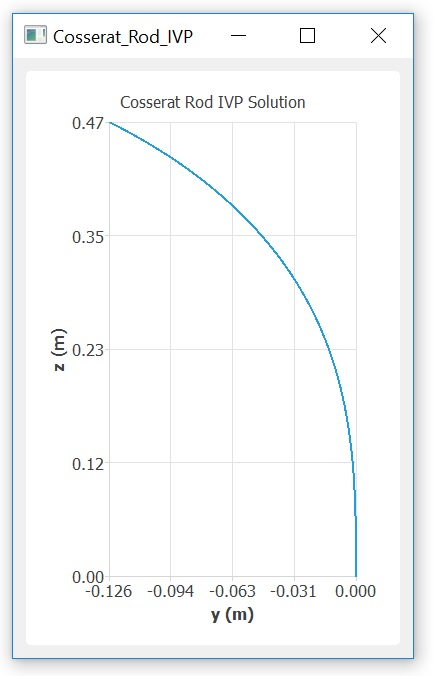
\includegraphics[width=0.5\textwidth]{fig/SolutionPlot.jpg}
	\label{fig:SolutionPlot}
\end{figure}
The ``plot'' command is defined in ``simpleplotting.h'' in the library folder. Qt has powerful visualization capabilities, but for many of the tutorials we'll abstract visualization to a single line if possible.

With this knowledge, we could find the shape of a rod given the position and orientation of where it was clamped and some 6-dof force sensor reading at the rod base.

\end{document}